\section{Diện tích hyperbolic và công thức Gauss-Bonnet}
Nhắc lại rằng diện tích của một tập con $A$ trong mặt phẳng Euclid $\R^2$ là 
\[\mu_{\R^2}(A) = \int_Adxdy.\]
Một cách tương tự, ta định nghĩa diện tích hyperbolic của một tập con $A$ trong mặt phẳng hyperbolic $\hh$. Tại mỗi $z\in \hh$, xét không gian vector tiếp xúc $T_z\hh$ trang bị tích vô hướng hyperbolic. Diện tích của hình bình hành sinh ra từ cơ sở chính tắc $e_1 = \begin{pmatrix}
    1\\0
\end{pmatrix},e_2 = \begin{pmatrix}
    0\\1
\end{pmatrix}$ là 
\[Vol_{hyp}(e_1,e_2) = \sqrt{\det\begin{pmatrix}
    \left<e_1,e_1\right>_{hyp} & \left<e_1,e_2\right>_{hyp}\\
    \left<e_2,e_1\right>_{hyp} & \left<e_2,e_2\right>_{hyp}
\end{pmatrix}} = \dfrac{1}{\im^2(z)}.\]
Điều này dẫn ta đến định nghĩa sau đây.
\begin{defn}
Diện tích hyperbolic của một tập con $A$ trong mặt phẳng hyperbolic $\hh$ là
\[\mu(A) = \mu_{\hh}(A) = \int_A\dfrac{dxdy}{y^2}\] 
nếu tích phân trên tồn tại.
\end{defn}

\begin{thm}
    Các phép đẳng cự thuộc $\PSL(2,\R)$ của $\hh$ bảo toàn diện tích hyperbolic. Cụ thể hơn, với mọi tập con $A \subset \hh$ và $f \in \PSL(2.\R)$ của $\hh$, ta có $\mu(f(A)) = \mu(A)$.
\end{thm}

\begin{proof}
    Giả sử $A \subset \hh$ và $\mu(A)$ tồn tại. 
    
    Lấy bất kỳ $f(z) = \dfrac{az+b}{cz+d} $ trong $\PSL(2,\R)$. Giả sử $f(z) = u(x,y)+iv(x,y)$. 
    
    Ta có
    \begin{align*}
        \mu(f(A)) = \int_{f(A)}\dfrac{dudv}{v^2}= \int_A{\dfrac{1}{v^2} |\det(Df(z))|dxdy}.
    \end{align*}
     Vì $f$ là hàm khả vi phức nên $\dfrac{\partial u}{\partial x} = \dfrac{\partial v}{\partial y} \text{ và } \dfrac{\partial u}{\partial y} = -\dfrac{\partial v}{\partial x}$. Suy ra 
     \[\left|\det(Df(z)\right| = \left|\det \begin{pmatrix}
                \dfrac{\partial u}{\partial x} & \dfrac{\partial u}{\partial y} \\
                 \dfrac{\partial v}{\partial x}& \dfrac{\partial v}{\partial y}
    \end{pmatrix}\right| = \left(\dfrac{\partial v}{\partial x}\right)^2 + \left(\dfrac{\partial v}{\partial y}\right)^2.\]
    Lại có $v = \im f(z) = \dfrac{\im z}{|cz+d|^2} = \dfrac{y}{(cx+d)^2 + c^2y^2}$ nên 
    \[\left(\dfrac{\partial v}{\partial x}\right)^2 + \left(\dfrac{\partial v}{\partial y}\right)^2 = \left(\dfrac{1}{(cx+d)^2 + c^2y^2}\right)^2.\]
    Từ đó ta được 
    \begin{align*}
        \mu(f(A)) 
        &= \int_A{\left(\dfrac{(cx+d)^2 + c^2y^2}{y}\right)^2 \left(\dfrac{1}{(cx+d)^2 + c^2y^2}\right)^2dxdy}
        = \int_A\dfrac{dxdy}{y^2} = \mu(A).
    \end{align*}
\end{proof}
\begin{defn}[Đa giác hyperbolic]
    Một đa giác hyperbolic $n-$cạnh trong $\hh$ là một tập con đóng của $\overline{\hh} = \hh \cup \R \cup \{\infty\}$, bị chặn bởi các đoạn trắc địa $[z_1,z_2],\ldots,[z_n,z_1]$. Các $z_i$ là giao của hai đoạn trắc địa của đa giác được gọi là đỉnh của đa giác hyperbolic đó.
\end{defn}
% \begin{exam*}
%     Lần lượt sau đây là các tam giác số đỉnh nằm trên $\R \cup \{\infty\}$ là $0,1,2,3$.
%     \begin{figure}[htp!]
%         \centering
%         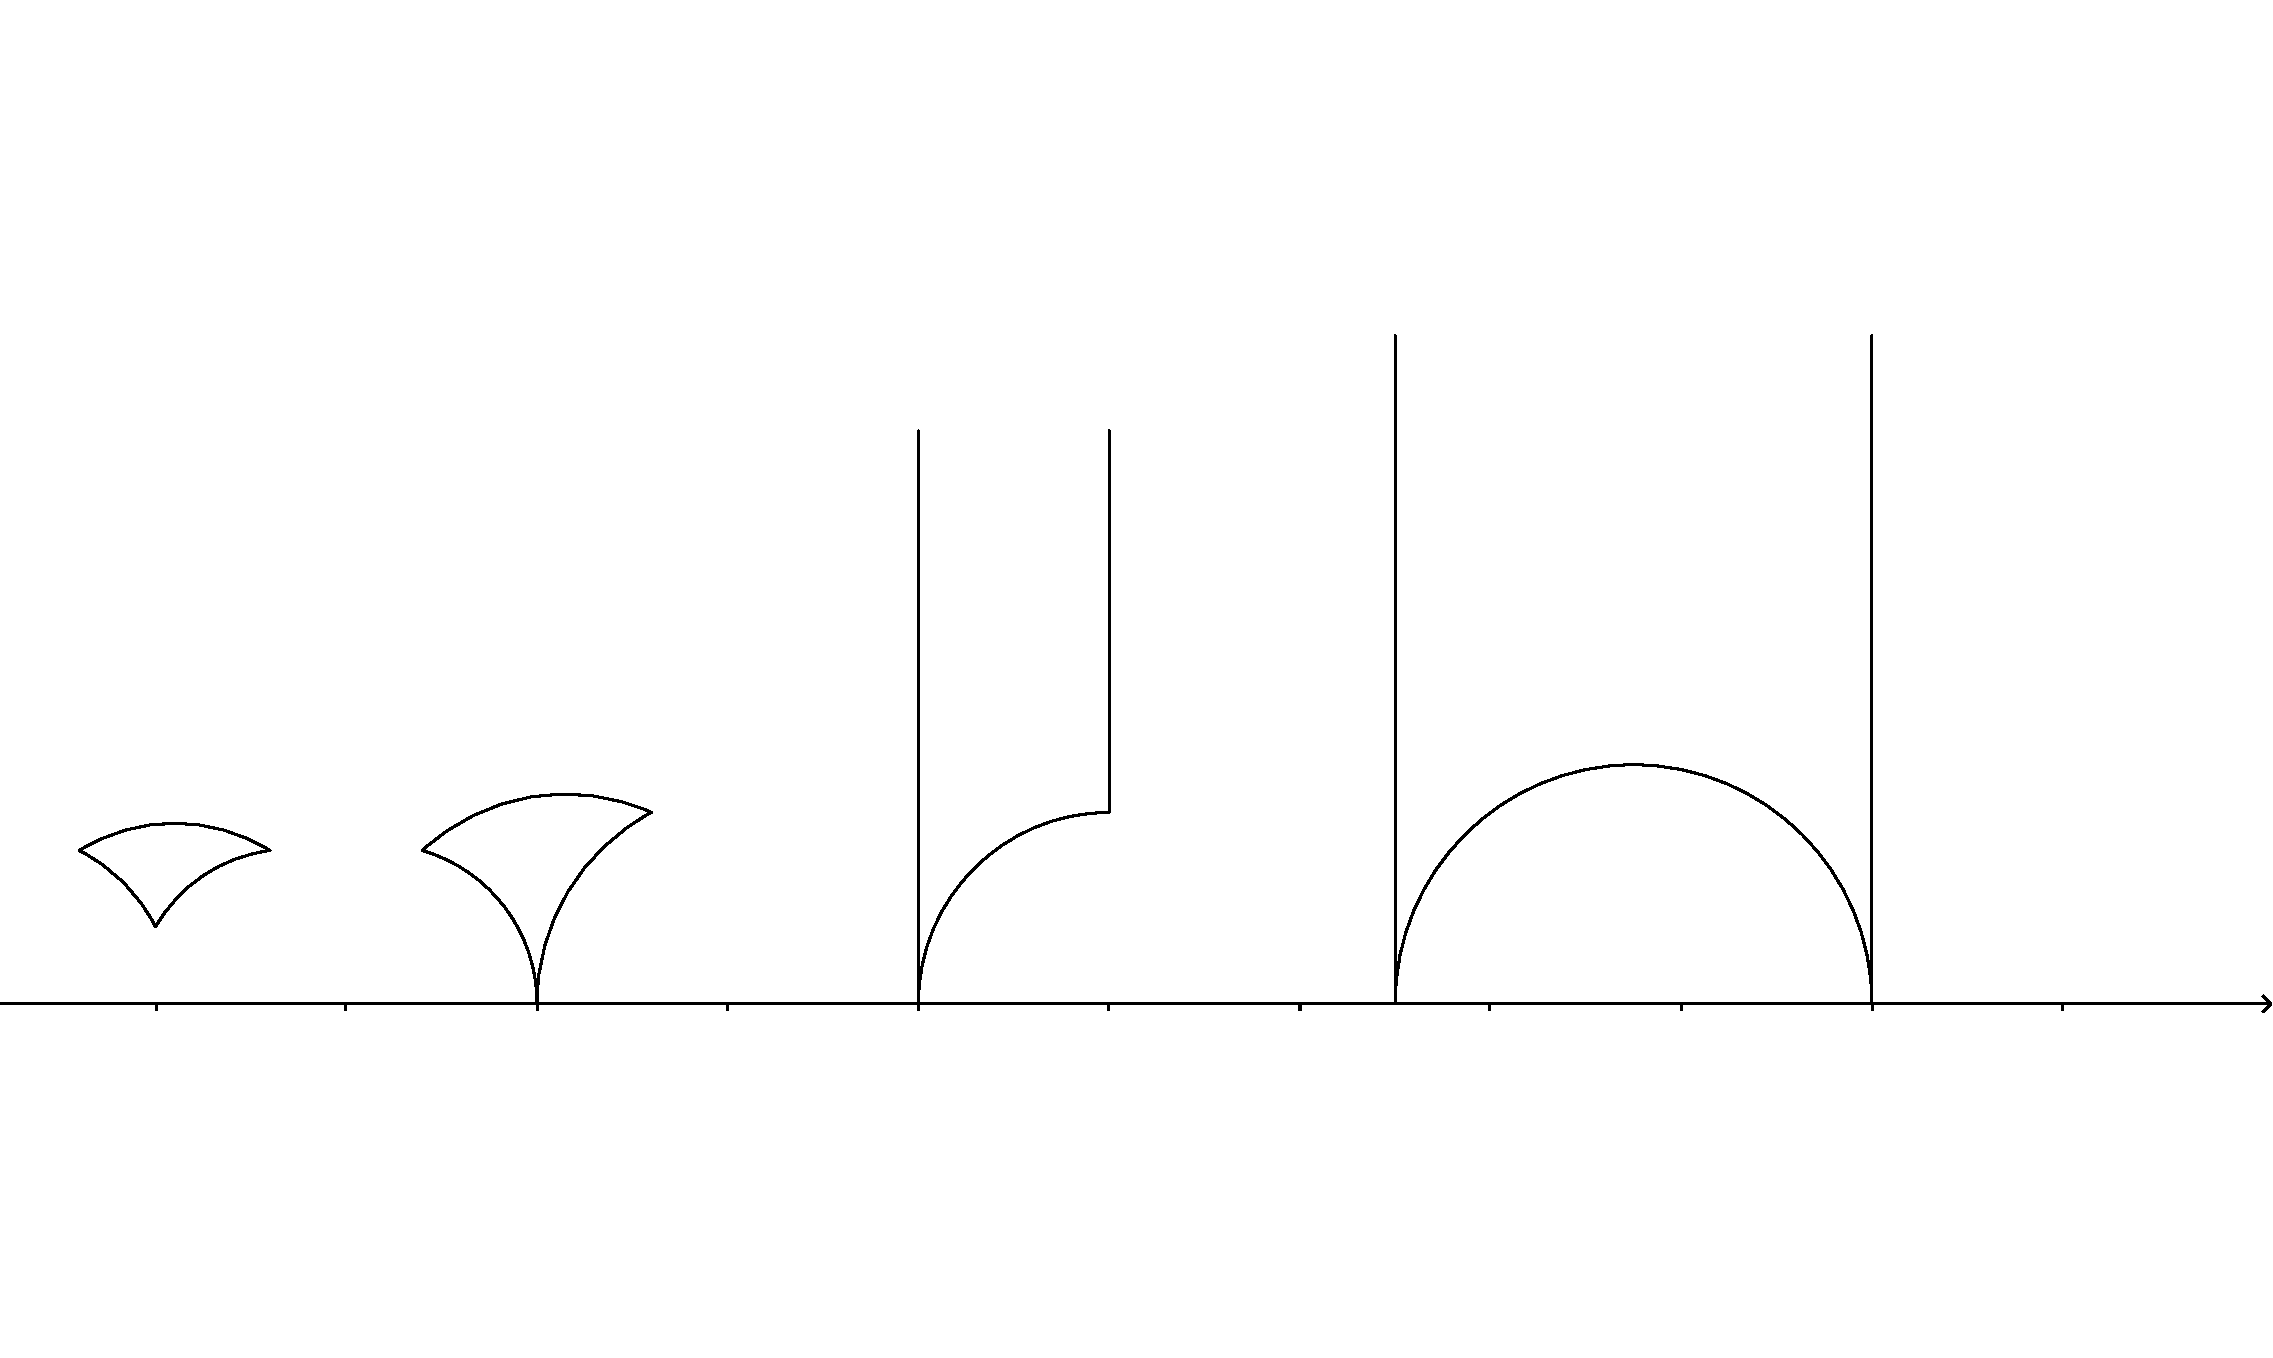
\includegraphics[width=0.7\linewidth]{images/polygon.pdf}
%         \caption{Tam giác hyperbolic}
%         \label{fig:enter-label}
%     \end{figure}
% \end{exam*}
Tiếp theo chúng ta đến với công thức Gauss-Bonnet để tính diện tích của tam giác hyperbolic.
\subsubsection{Định lý Gauss-Bonnet}
\begin{thm}[Gauss-Bonnet]\label{thm 2.4.5}
    Cho $\Delta$ là một tam giác hyperbolic với các góc $\alpha, \beta, \gamma$. Khi đó \[\mu(\Delta) = \pi - (\alpha + \beta + \gamma).\]
\end{thm}
\begin{proof}
    Giả sử $\Delta$ là một tam giác hyperbolic có các đỉnh lần lượt là $A,B,C \in \overline{\hh} = \hh \cup \R\cup \{\infty\}$ và các góc tương ứng các đỉnh lần lượt là $\alpha,\beta, \gamma$. 

    Khi đó ta có các trường hợp sau
    \begin{enumerate}
        \item $\Delta$ có một trong 3 đỉnh thuộc $\R \cup \{\infty\}$. 
        
        Không mất tính tổng quát, ta có thể giả sử $A, B \in \hh$, $C = \infty$.
        
        Vì nếu $C = r \in \R$. Xét phép biến đổi $T(z) = \dfrac{-1}{z-r}$ trong $\PSL(2,\R)$. Qua tác động của $T$ thì $T(A),T(B) \in \hh$ và $T(C) = \infty$. Mà $T$ bảo toàn diện tích hyperbolic và cũng bảo toàn góc trong $\hh$ nên \[\mu(T(A)T(B)T(C)) = \mu(\Delta).\]
        Khi đó trắc địa qua $A, \infty$ và trắc địa qua $B,\infty$ sẽ là các đường hyperbolic vuông góc với trục thực. Còn trắc địa qua $A,B$ là một nửa đường tròn vuông góc với trục thực.
        
        Bằng cách tác động một cách phù hợp các đẳng cự có dạng $z\mapsto z+k,k\in \R$ hoặc $z\mapsto \lambda z, \lambda>0$ trong $\PSL(2,\R)$, mà vẫn bảo toàn diện tích hyperbolic cũng như bảo toàn góc. Ta có thể giả sử trắc địa qua $A,C$ là $h-line(a,\infty)$, trắc địa qua $B,C$ là $h-line(b,\infty)$ và trắc địa qua $A,B$ là $h-line(-1,1)$. 

        \begin{figure}[htp!]
            \centering
            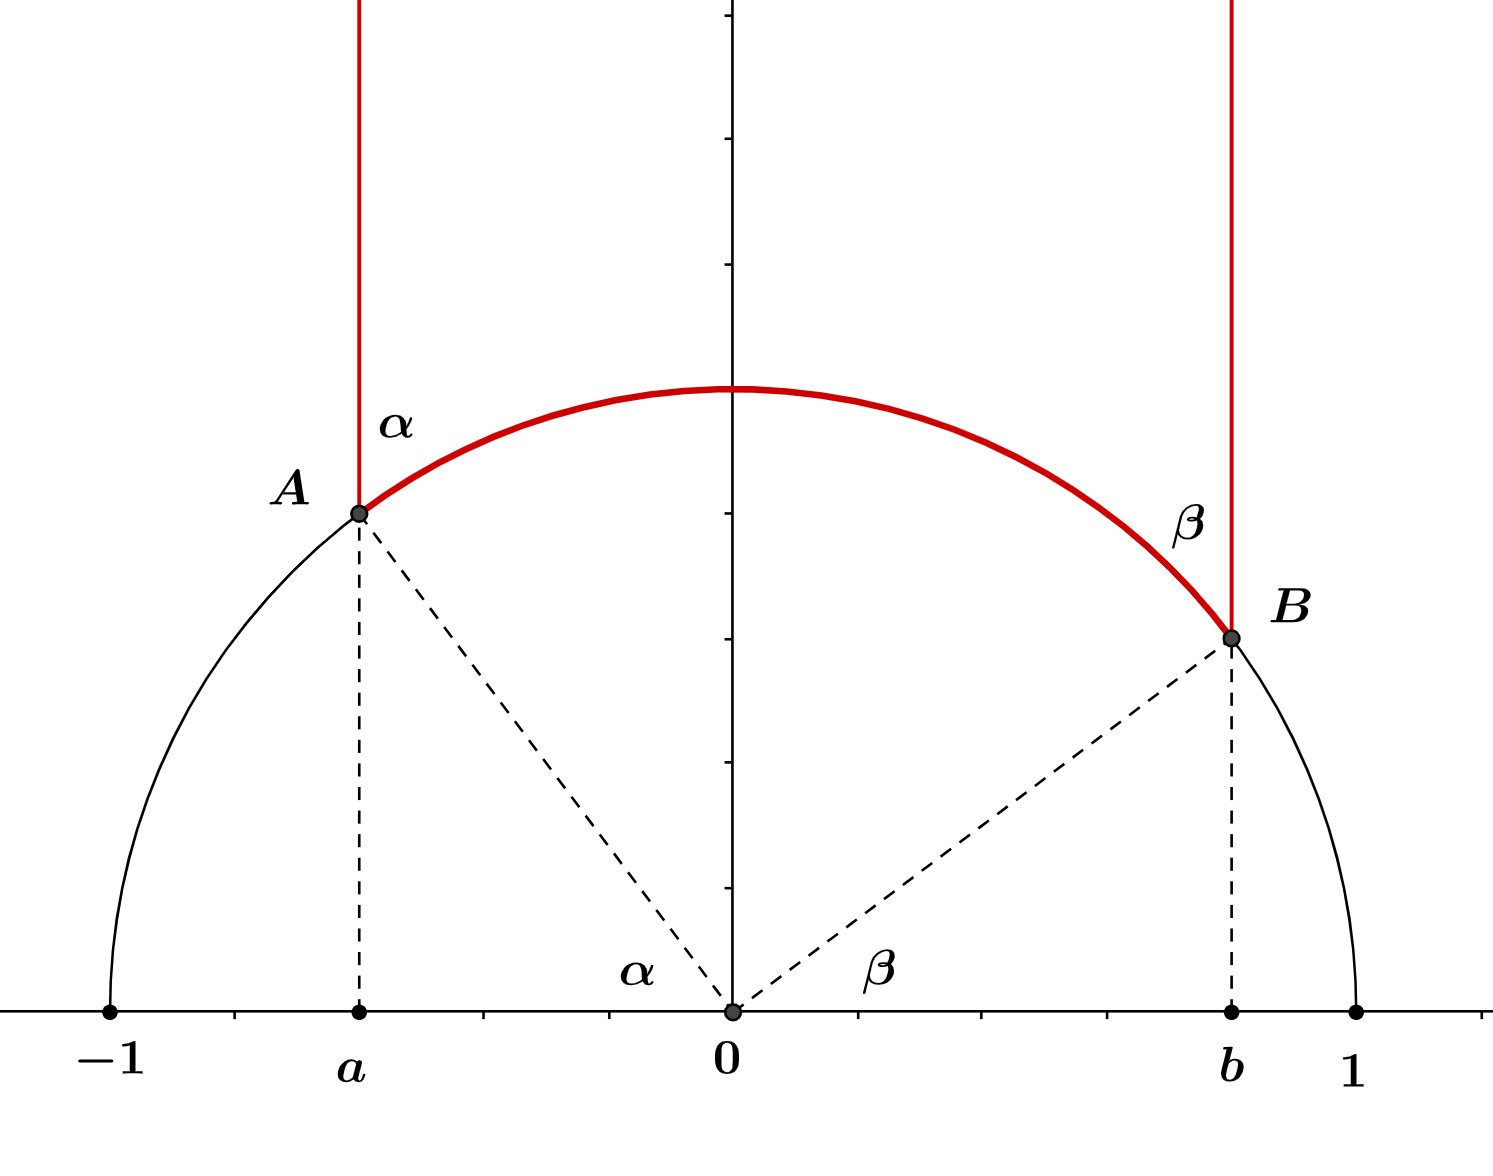
\includegraphics[width=0.4\linewidth]{images/Gauss-Bonnet_1.png}
            % \caption{}
            % \label{fig:enter-label}
        \end{figure}
        Đường cong tham số qua $A,B$ là $y = \sqrt{1-x^2}, a \leq x \leq b$. 
        Do đó \begin{align*}
            \mu(\Delta) = \int_{\Delta}{\dfrac{dxdy}{y^2}} = \int_a^b{dx}\int_{\sqrt{1-x^2}}^{\infty}{\dfrac{dy}{y^2}} = \int_a^b{\dfrac{dx}{\sqrt{1-x^2}}}.
        \end{align*}
        Đặt $x = \cos\theta$ với $\theta \in [0,\pi]$. Khi đó 
        \[\mu(\Delta) = \int_{\pi-\alpha}^{\beta}{\dfrac{-\sin\theta d\theta}{\sin\theta}} = \pi -\alpha -\beta=\pi-(\alpha + \beta + \gamma)~(\text{vì }\gamma = 0).\]

        \item $\Delta$ không có đỉnh nào trong $\R \cup \{\infty\}$.

        Ta có thể tác động các phép biến đổi trong $\PSL(2,\R)$ sao cho trắc địa qua các cạnh của $\Delta$ đều là các nửa đường tròn vuông góc với trục thực. Giả sử trắc địa qua $A,C$ cắt trục thực tại $D$. Kí hiệu $\Delta_1$ là tam giác hyperbolic có 3 đỉnh là $A,B,D$ và $\Delta_2$ là tam giác hyperbolic có 3 đỉnh là $B,C,D$, hai tam giác này đều có 1 đỉnh trên $\R\cup\{\infty\}$ và 2 đỉnh còn lại trên $\hh$. Áp dụng công thức tính diện tích của chúng như trường hợp 1 ta được
        \begin{figure}
            \centering
            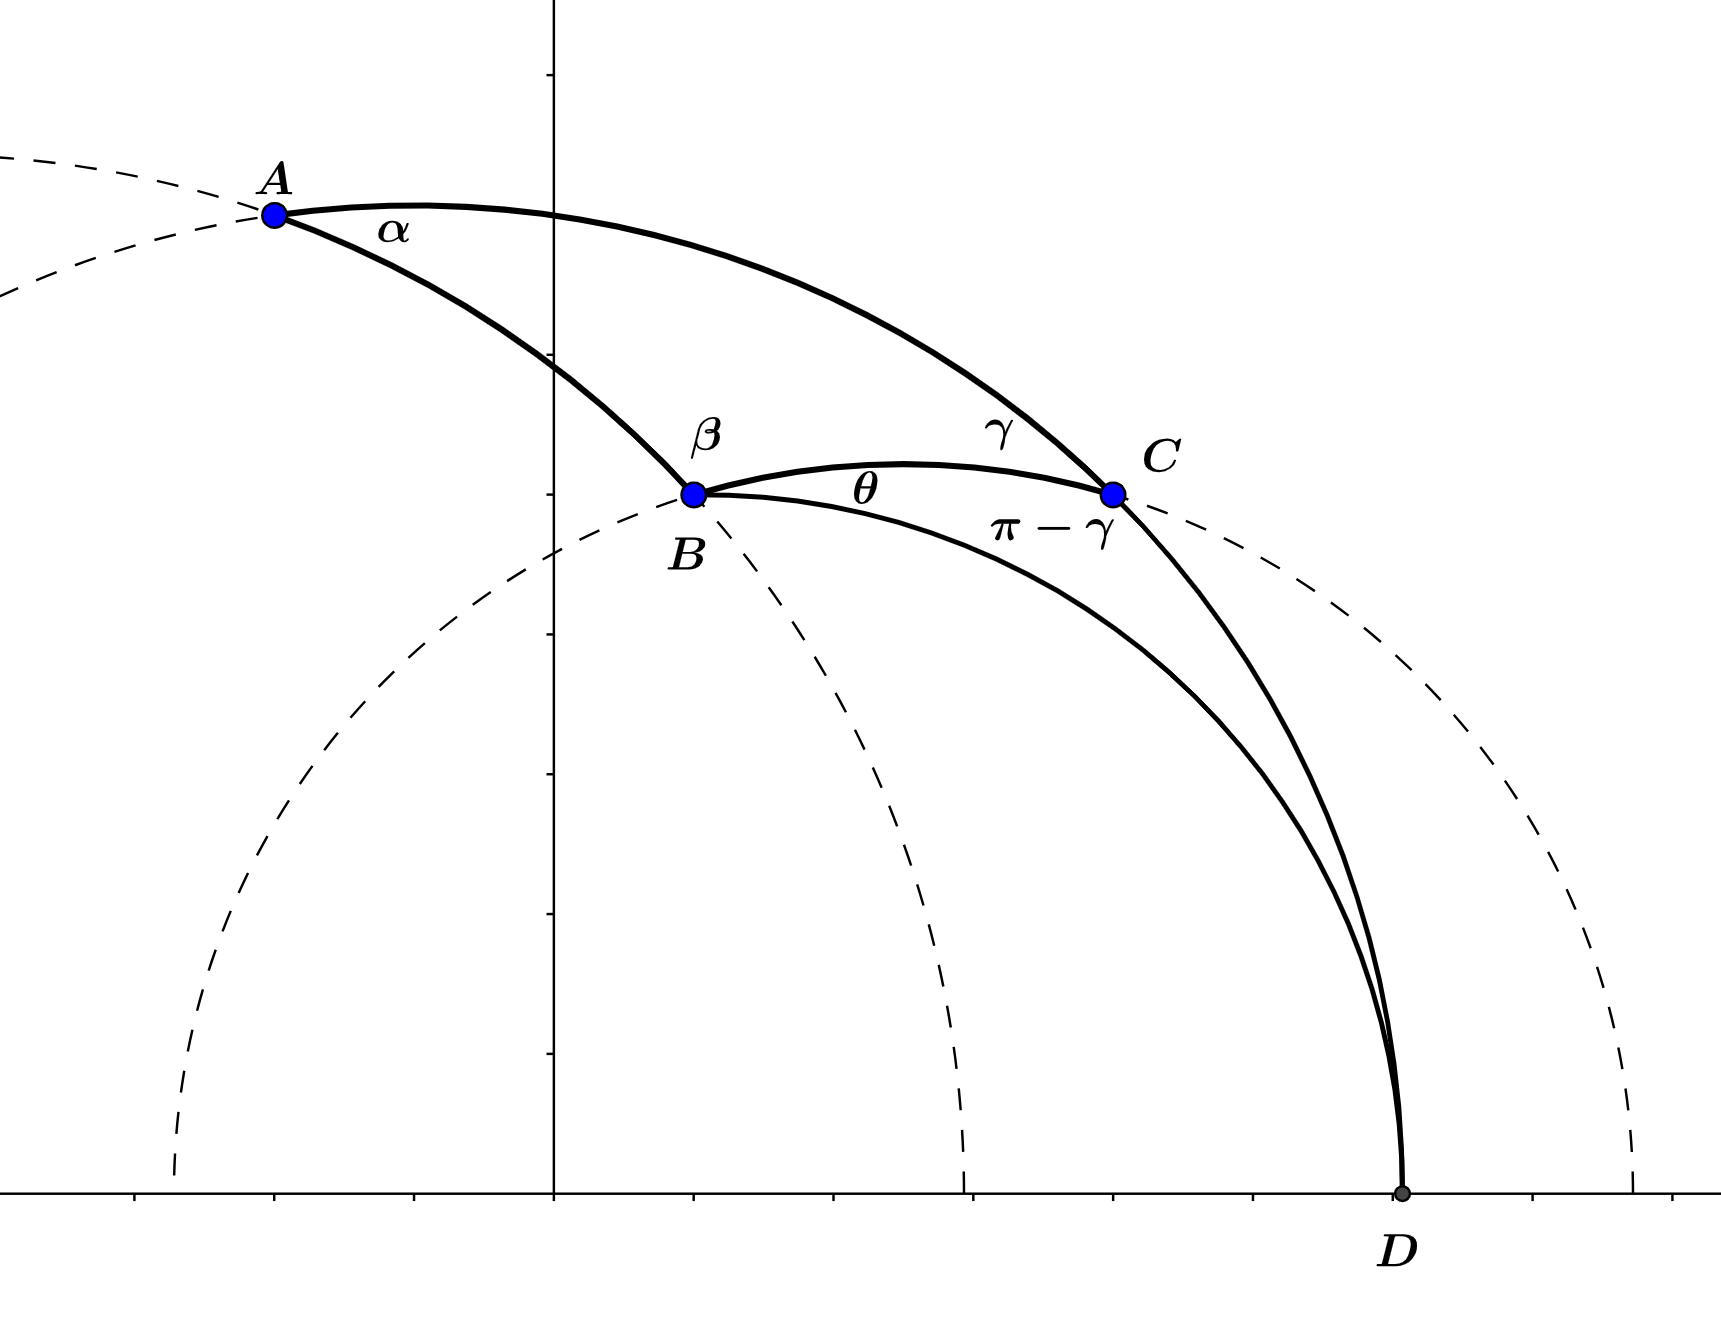
\includegraphics[width=0.4\linewidth]{images/gauss-bonnet-2.png}
            % \caption{Enter Caption}
            % \label{fig:enter-label}
        \end{figure}
        \[\mu(\Delta) = \mu(\Delta_1) -\mu(\Delta_2) = [\pi - (\alpha)-(\beta + \theta)] - [\pi - (\theta + \pi -\gamma)] = \pi -\alpha - \beta -\gamma.\]
        
        \item $\Delta$ có hai đỉnh trong $\R \cup \{\infty\}$ và đỉnh còn lại thuộc $\hh$.
    
        Giả sử $A \in \hh, B \in \R$ và $C = \infty$ (còn trường hợp $A \in \hh,~B,C \in \R$, ta có thể tác động một đẳng cự biến $B\mapsto \infty$). Khi đó $\beta =0 = \gamma$ và 
        \[\mu(ABC) = \mu(ABD) + \mu(ADC) = \pi-(\theta+\phi) + \pi -(\alpha - \theta) - (\pi-\phi) = \pi - \alpha = \pi-(\alpha + \beta + \gamma).\]

        \begin{figure}[htp!]
        \centering
        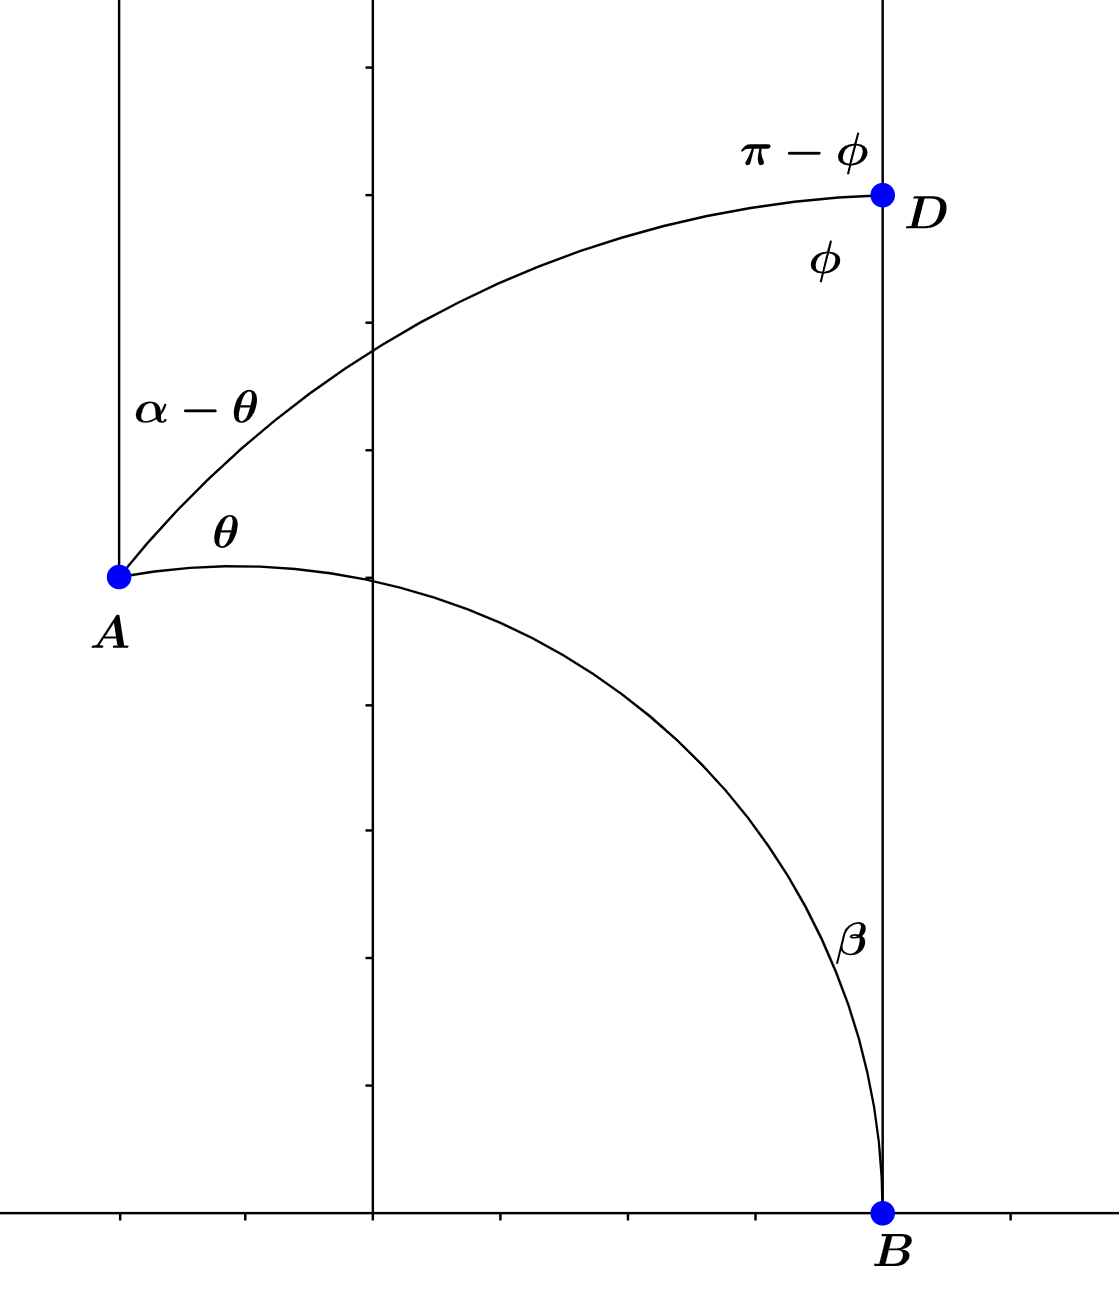
\includegraphics[width=0.3\linewidth]{images/Gauss-Bonnet_3.png}
        % \caption{Enter Caption}
        % \label{fig:enter-label}
        \end{figure}
    \item $\Delta$ có 3 đỉnh trên $\R \cup \{\infty\}$.

        Giả sử $A,B \in \R, C = \infty$ (nếu $A,B,C \in \R$, bằng đẳng cự có dạng $z \mapsto \dfrac{-1}{z-k}$ phù hợp ta có thể đưa một trong 3 đỉnh trên thành $\infty$).
        
        Khi đó, bằng tác động phép đẳng cự phù hợp có dạng $z\mapsto z+k$, ta có thể giả sử trắc địa qua $A,C$ là $h-line(-a,\infty)$, trắc địa qua $B,C$ là $h-line(a,\infty)$ và đẳng cự qua $A,B$ là $h-line(-a,a)$.
        \begin{figure}[htp!]
        \centering
        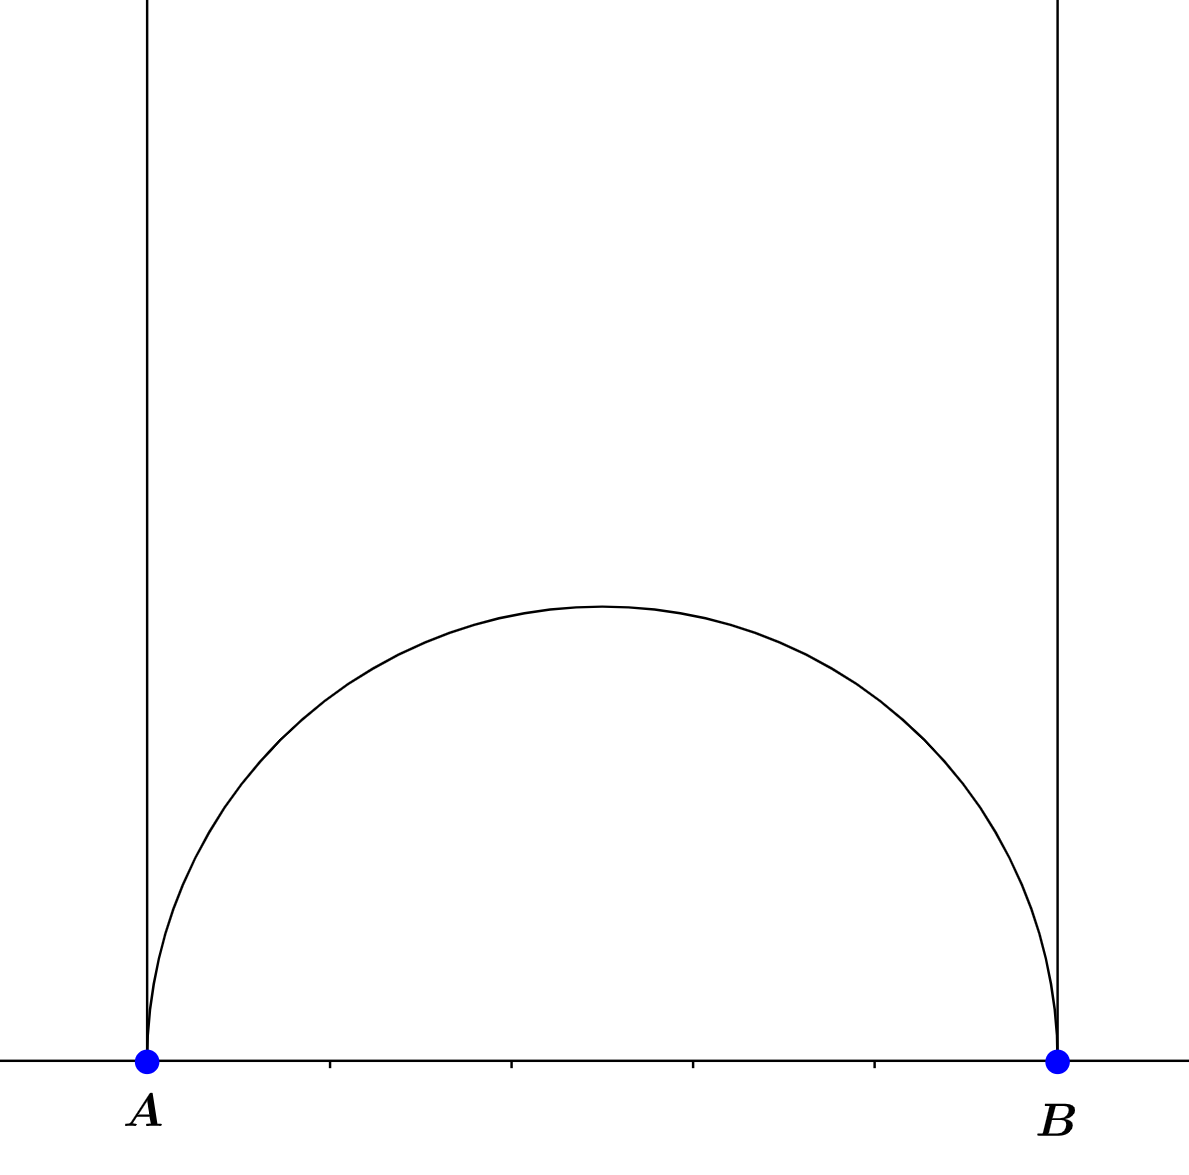
\includegraphics[width=0.3\linewidth]{images/Gauss-Bonnet_4.png}
        % \caption{Enter Caption}
        % \label{fig:enter-label}
        \end{figure}
        Do đó $\alpha = \beta =\gamma = 0$ và 
        \begin{align*}
            \mu(\Delta) = \int_{\Delta}{\dfrac{dxdy}{y^2}} = \int_{-a}^a{dx}\int_{\sqrt{a^2-x^2}}^{\infty}{\dfrac{dy}{y^2}} = \int_{-a}^a{\dfrac{dx}{\sqrt{a^2-x^2}}} = \pi = \pi -(\alpha+\beta + \gamma).
        \end{align*}
    \end{enumerate}
    Vậy ta luôn có $\mu(\Delta) = \pi -(\alpha+\beta + \gamma).$
\end{proof}
